\chapter{Experimental Setup and Datasets}
\label{chap:Experiment}

Let us introduce the experimental setup first: in this chapter, we discuss the detector and its data acquisition system,
along with some data preprocessing. Then, we present the data distribution we have been working with and used to
test our data quality monitoring algorithm.

\section{Drift tube detector}
\label{s:DriftTube}

The whole detector consists of four muon chambers, also called superlayers (SLs). Each muon chamber comprises 64
drift tubes (DTs), grouped into four staggered layers of 16 drift cells. A visual representation of the detector
configuration is shown in \autoref{fig:detector}, in which only 20 out of 64 DTs have been reported. The transverse
cross-section of the drift cells is $L \times h = 42 \times 13 \,\si{\mm}^2$ and they are filled with an
$\text{Ar-CO}_{2}$ ($85/15\%$) gas mixture at $1\,\text{atm}$. Each DT contains an anodic wire at a high voltage
potential ($V_{\text{wire}}=+3600\,\si{\volt}$), while the sidewalls of the tubes are cathodes at
$V_{\text{cathod}}=-1800\,\si{\volt}$. Furthermore, two additional electrodes at $V_{\text{strip}}=-1200\,\si{\volt}$
are placed on the top and bottom wall of the tube to ensure the uniformity of the electric field inside the cell. 

\begin{figure}[H]
    \centering
    \definecolor{myfill}{RGB}{255, 187, 187}
\definecolor{mycolor}{RGB}{255, 17, 17}
\definecolor{absred}{RGB}{255, 0, 0}

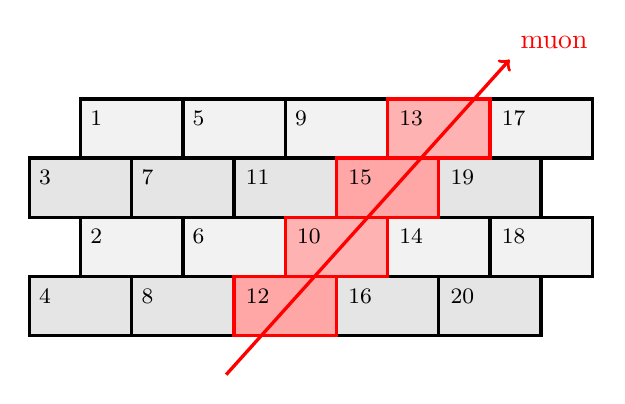
\begin{tikzpicture}

    % lower layer
    \filldraw[color=black, fill=black!10, very thick] (0.0,0.0) rectangle + (1.3,0.75);
    \filldraw[color=black, fill=black!10, very thick] (1.3,0.0) rectangle + (1.3,0.75);
    
    \filldraw[color=black, fill=black!10, very thick] (3.9,0.0) rectangle + (1.3,0.75);
    \filldraw[color=black, fill=black!10, very thick] (5.2,0.0) rectangle + (1.3,0.75);

    \node at (0.2,0.5) {\footnotesize $4$}; 
    \node at (1.5,0.5) {\footnotesize $8$};
    
    \node at (4.2,0.5) {\footnotesize $16$};
    \node at (5.5,0.5) {\footnotesize $20$};
 
    % second layer
    \filldraw[color=black, fill=black!5, very thick] (0.65,0.75) rectangle + (1.3,0.75);
    \filldraw[color=black, fill=black!5, very thick] (1.95,0.75) rectangle + (1.3,0.75);
    \filldraw[color=black, fill=black!5, very thick] (3.25,0.75) rectangle + (1.3,0.75);
    \filldraw[color=black, fill=black!5, very thick] (4.55,0.75) rectangle + (1.3,0.75);
    \filldraw[color=black, fill=black!5, very thick] (5.85,0.75) rectangle + (1.3,0.75);

    \node at (0.2+0.65,0.5+0.75) {\footnotesize $2$}; 
    \node at (1.5+0.65,0.5+0.75) {\footnotesize $6$};
    
    \node at (4.2+0.65,0.5+0.75) {\footnotesize $14$};
    \node at (5.5+0.65,0.5+0.75) {\footnotesize $18$};

    % third layer
    \filldraw[color=black, fill=black!10, very thick] (0.0,1.5) rectangle + (1.3,0.75);
    \filldraw[color=black, fill=black!10, very thick] (1.3,1.5) rectangle + (1.3,0.75);
    \filldraw[color=black, fill=black!10, very thick] (2.6,1.5) rectangle + (1.3,0.75);
    
    \filldraw[color=black, fill=black!10, very thick] (5.2,1.5) rectangle + (1.3,0.75);

    \node at (0.2,2.0) {\footnotesize $3$}; 
    \node at (1.5,2.0) {\footnotesize $7$};
    \node at (2.9,2.0) {\footnotesize $11$};
    
    \node at (5.5,2.0) {\footnotesize $19$};

    % upper layer
    \filldraw[color=black, fill=black!5, very thick] (0.65,2.25) rectangle + (1.3,0.75);
    \filldraw[color=black, fill=black!5, very thick] (1.95,2.25) rectangle + (1.3,0.75);
    \filldraw[color=black, fill=black!5, very thick] (3.25,2.25) rectangle + (1.3,0.75);

    \filldraw[color=black, fill=black!5, very thick] (5.85,2.25) rectangle + (1.3,0.75);

    \node at (0.2+0.65,2.0+0.75) {\footnotesize $1$}; 
    \node at (1.5+0.65,2.0+0.75) {\footnotesize $5$};
    \node at (2.8+0.65,2.0+0.75) {\footnotesize $9$};
    
    \node at (5.5+0.65,2.0+0.75) {\footnotesize $17$};
       
    % muon track
    \filldraw[color=red, fill=red!30, very thick] (4.55,2.25) rectangle + (1.3,0.75);
    \node at (4.2+0.65,2.0+0.75) {\footnotesize $13$};

    \filldraw[color=red, fill=red!35, very thick] (3.9,1.5) rectangle + (1.3,0.75);
    \node at (4.2,2.0) {\footnotesize $15$};

    \filldraw[color=red, fill=red!30, very thick] (3.25,0.75) rectangle + (1.3,0.75);
    \node at (2.9+0.65,0.5+0.75) {\footnotesize $10$};

    \filldraw[color=red, fill=red!35, very thick] (2.6,0.0) rectangle + (1.3,0.75);
    \node at (2.9,0.5) {\footnotesize $12$};

    \draw[color=red, very thick, ->] (2.5,-0.5) -- (6.1,3.5) node[above right] {muon};
     



        
\end{tikzpicture}
    \captionof{figure}{Detector staggered layers configuration}
    \label{fig:detector}
\end{figure}  

The active volume of the detector is the gas mixture, which gets ionized by ionizing particles. Electrons
knocked off the gas, surrounded by the uniform electric field as described above, drift towards the anodic wire at an
almost constant velocity of $v_{\text{drift}} \approx 54 \,\si{\um}/\si{\ns}$. As the electrons reach the wire, the
deposit of electric charge produces an electrical signal. The actual quantity being measured is the time $t$ of the
electric signal detection, from which one could extrapolate information about the muon arrival time and the drift time
$t_{\text{d}}$. The drift time corresponds to the time taken by the electrons to reach the anodic wire and, since the
uniformity of the electric field leads to a constant drift velocity $v_{\text{drift}}$, one could easily compute the
distance, which we call $x$, between the hit position of the muon and the wire. 
\begin{equation}\label{eq:x}
    x = v_{\text{d}} \times t_{\text{d}} = v_{\text{d}} \times (t - t_{\text{0}})
\end{equation}

As shown in \autoref{eq:x}, in order to compute the drift time $t_{\text{d}}$, a time pedestal $t_{0}$ should be
subtracted from the detection time $t$: such $t_{0}$ is a parameter holding contributions from both trigger time and
electronics delay in detecting and collecting data.



\section{Data acquisition and format}
\label{s:DataFormat}

The electric charge accumulated on the anodic wire is amplified, shaped and discriminated given a predefined threshold
by the front-end (FE) electronics located within the active volume of the tubes. Signals above the discriminating
threshold are sent to two FPGAs that implement the time-to-digital conversion (TDC), assigning each activated channel a
time value $t$. A pair of scintillator tiles provide an external timing reference. It is noticeable that a single FPGA
can digitize the entirety of the channels from two muon chambers, and the additional TDCs available are used for
digitizing external signals such as the scintillator. In addition, an external oscillator generates a clock signal, sent
to both FPGAs: to emulate CERN TTC Systems a $40\,\si{\mega\hertz}$ clock, compatible with the bunch crossing (BX)
frequency at LHC, is generated.

Practically speaking, the time-stamp $t$ returned by the TDC corresponds to the rising edge of the input signal with
respect to the rising edge of the clock. On top of that, an appropriate counter assigns to each TDC measurement its
corresponding BX counter: the granularity of the time measures is thus $1/30$ of BX. Finally, another counter, related
to the orbit of protons around the accelerator ring at LHC, is assigned to each BX. The final result is a time
measurement format similar to standard time (hours : minutes : seconds), and the conversion to nanoseconds is given by 

\begin{equation}\label{eq:time_conversion}
    t = \text{ORBIT\_CNT} \times 3564 \times 25 + \text{BX\_COUNTER} \times 25 + \text{TDC\_MEAS} \times 25/30
\end{equation}

The raw data is then preprocessed to produce .txt files having as rows all the collected signals above the
discriminating threshold and as columns the following features:

\begin{itemize}
    % \itemsep1em
    \item \textbf{HEAD} \\ Additional information discriminating different kinds of data. 
    \item \textbf{FPGA} \\ Specifies which of the two FPGAs collected the signal.
    \item \textbf{TDC\_CHANNEL} \\ Integer value in the interval $[0,\,127]$ referring to the FPGA channels.
    \item \textbf{ORBIT\_CNT} \\ Integer in the interval $[0,\,2^{32}]$. 
    \item \textbf{BX\_COUNTER} \\ Integer in the interval $[0,\,3564]$. 
    \item \textbf{TDC\_MEAS} \\ Integer in the interval $[1,\,30]$.
\end{itemize}

The first feature is only used to discriminate between relevant data and unnecessary data. For example, the experiment
has other triggers, and their signals are stored in the same data file and distinguished by a different HEAD tag. The
detector itself is a great case study for many different works of experimental physics, but of course, not all data is
necessary for every kind of task we want to tackle. The second and third feature, instead, allows for tracking which
drift tube has collected the signal: the FPGA tag (either $0$ or $1$) locates the muon chambers in pairs (each FPGA
board is connected to two superlayers), while the TDC\_CHANNEL, meaning the channel of the FPGA, locates the drift tube.
Finally, the last three features hold the timing information as described above.  \\

Note that a more detailed description of the experimental setup, namely the detector and its electronic chain, is
accurately reported in \cite{migliorini}. However, as it is not crucial to our work, we do not elaborate further on the
experimental setup in this thesis.

\section{The drift time distribution}
\label{s:DriftTime}

The distribution we are interested in monitoring is the distribution of drift times. It is the collection of time taken
by electrons to drift towards the wire at the center of the DTs. As mentioned in \autoref{s:DriftTube}, in order to
compute the drift time $t_{\text{d}}$ we need to follow a few steps. The trigger-less acquisition system reads the
sensors every $25\,\si{\ns}$ and each signal above the predefined threshold is recorded. Thus we first need to
discriminate events from background signals.

We define an \textit{event} as the collection of all the electric signals produced by a muon crossing the detector.
Since one orbit (the \textit{ORBIT\_CNT} counter) corresponds to approximately $90\,\si{\us}$, the actual probability of
having two muons traversing the detector within the same orbit is low. Thus, we can assume that all the hits that have
the same \textit{ORBIT\_CNT} value of an external trigger signal can be gathered into an \textit{event}. The external
trigger used is the scintillator, characterized by the special channel $128$ of the second FPGA. 

Once all the events within the dataset have been discriminated from the background noise, we need to convert the
time-stamp values (assigned by the TDC) into nanoseconds using \autoref{eq:time_conversion}. We will call the
scintillator time stamp, expressed in nanoseconds, as $t_{\text{scint}}$. Then, as stated in \autoref{s:DriftTube}, to
compute the Drift Time of one hit, we should subtract the time pedestal $t_{0}$ from the hit time $t$:

\begin{equation}\label{eq:td}
    t_{\text{d}}=t-t_{0}=t-(t_{\text{scint}}+\text{scint\_offset}+\text{SL\_offset})
\end{equation}

\noindent where $\text{scint\_offset}$ is related to electronics delays while $\text{SL\_offset}$ follows from the
geometry of the detector, as muons pass through the superlayers with different times depending on the particle track.

Drift time distributions are expected to be uniform, ranging between $0\,\si{\nano\second}$ and approximately
$400\,\si{\nano\second}$, and they are often referred to as \textit{time boxes}. Hence, by plotting the
$t-t_{\text{scint}}$ distribution we find the overall offset, composed by the last two terms if \autoref{eq:td}, by
shifting the distribution to have the rising edge at roughly $0\,\si{\nano\second}$. An example is shown in
\autoref{fig:dt_distribution}, in which the offset has been roughly calculated to be $100\,\si{\nano\second}$. A more
accurate and comprehensive study on the calibration of the time pedestals is reported in both \cite{amapane} and
\cite{cmscolab}: although these articles refer to the CMS's muon chambers, a similar procedure can be implemented to
accurately compute the calibration constants. For our purposes, however, a rough calibration is sufficient to prevent
the procedure from failing.

\begin{figure}[h]
    \centering
    \includegraphics[width=0.7\textwidth]{./Images/experiment/RUN1252_both.pdf}
    \caption{Example of a drift time distribution before and after tuning the offset parameter}
    \label{fig:dt_distribution}
\end{figure}

Among plenty of different distributions, we have chosen to work with drift times as the shape of the time box is
strictly related to the correct functioning of the detector. Numerous disparate factors can affect that distribution,
from the data acquisition system to the DTs gas mixture proportions, pressure and more. Thus, if the detector is working
as expected, the drift time distribution should look like the one in \autoref{fig:dt_distribution}. On the other hand, a
detector failure leads to a time box with different widths or discrepancies in the edges and tails.


